Машинное обучение предполагает построение математических моделей, помогающих понять данные. "Обучение" вступает в игру, когда мы даем этим моделям настраиваемые параметры, которые могут быть адаптированы к наблюдаемым данным; таким образом, программу можно считать " обученной" на основе данных. После того, как эти модели подогнаны под ранее наблюдаемые данные, их можно использовать для прогнозирования и понимания аспектов вновь наблюдаемых данных.

\subsubsection{Категории машинного обучения}\label{ml}
На самом фундаментальном уровне машинное обучение можно разделить на два основных типа: обучение с учителем и без него.

%здесь график с методами машинного обучения

Обучение с учителем включает в себя некое моделирование взаимосвязи между измеряемыми характеристиками данных и некоторой маркировкой, связанной с данными; после определения этой модели она может быть использована для нанесения меток на новые, неизвестные данные. Далее это подразделяется на задачи классификации и регрессионные задачи: в классификации метки являются дискретными категориями, а в регрессии - непрерывными величинами. 

% side by side регрессия и классификация

Обучение без учителя включает в себя моделирование свойств данных без привязки к какой-либо метке, и часто описывается как "позволить данным говорить самим за себя". Эти модели включают такие задачи, как кластеризация и уменьшение размерности. Алгоритмы кластеризации идентифицируют различные группы данных, в то время как алгоритмы уменьшения размерности ищут более сжатые представления данных.

% кластеризация

Кроме того, существуют так называемые методы с частичным привлечением учителя, которые находятся где-то между обучением под наблюдением и обучением без наблюдения. Методы с частичным привлечением учителя часто бывают полезны, когда метки имеются лишь для части данных.


\subsection{Нейронные сети} \label{neuralnets}
Попытки воспроизвести способность биологических нервных систем обучаться и исправлять ошибки привели к созданию искусственных нейронных сетей. Искусственные нейронные сети представляют собой семейство моделей, построенных по принципу организации и функционирования биологических нейронных сетей — сетей нервных клеток живого организма.


Понятие искусственной нейронной сети было предложено ещё в 1943 году У. Маккалоком и У. Питтсом в статье \cite{neural_nets}. В частности, ими была предложена модель искусственного нейрона.
Чтобы отразить суть биологических нейронных систем, искусственный нейрон строится следующим образом. Он получает входные сигналы (исходные данные либо выходные сигналы других нейронов нейронной сети) через несколько входных каналов. Каждый входной сигнал проходит через соединение, имеющее определенный вес. С каждым нейроном связано определенное пороговое значение. Вычисляется взвешенная сумма входов, из нее вычитается пороговое значение и в результате получается величина активации нейрона . Сигнал активации преобразуется с помощью функции активации и в результате получается выходной сигнал нейрона.
На Рис.\ref{neuron} приведен пример искусственного нейрона.

\begin{figure}[h]
    \centering
    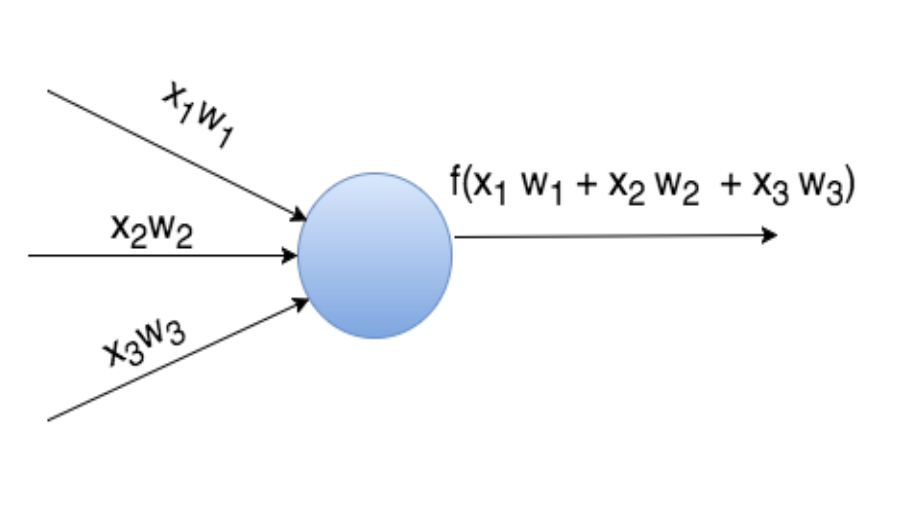
\includegraphics [width=\textwidth*2/3] {images/neuron.png}
    \caption{Искусственный нейрон}
    \label{fig:neuron}
\end{figure}

$x_i$ - входной сигнал
$w_i$ - вес входного сигнала $f(*)$- функция активации

\subsubsection{Функции активации}
В данном разделе описаны используемые в работе функций активаций для нейонных сетей.
\begin{itemize}
    \item Сигмоидная: $f(x) = \dfrac{1}{1-e^{-x}}$
    \item Линейная: $f(x) = x$
    \item Положительно линейная (ReLU): $f(x) = max(0, x)$
    \item  Софтмакс (Softmax): $f(x)j = \dfrac{e^{s_j}}{\sum^K_{k=1}e^{s_k}}$, для $j = 1, .., K$
\end{itemize}

\subsubsection{Функция потерь}
Введем обозначения: $X$— множество описаний объектов, $Y$ — множество допустимых ответов. Предполагается, что существует неизвестная целевая зависимость — отображение $y* : X \rightarrow Y$ , значения которой известны только на объектах конечной обучающей выборки 
$X^m = \begin{matrix}\{ (x_1, y_1), & ..., & (x_m, y_m)  \}\end{matrix}$.

Вводится функция потерь $L(y, y')$, характеризующая величину отклонения ответа $y$ от правильного ответа $y' = y^*(x)$ на произвольном объекте $x \in X$. Тогда эмпирический риск \cite{classification} — функционал качества, характеризующий среднюю ошибку на обучающей выборке:
\[
    Q(a,X^m)= \dfrac{1}{m} \sum^m_{i=1} L(y_i,y^*(x_i))
\]
В процессе обучения нейронная сеть настраивает веса $W$, минимизируя эмпирический риск.

При решении задачи многоклассовой классификации на выходе нейронной сети необходимо получить вероятность принадлежности объекта каждому из классов. В этом случае в качестве функции потерь обычно используется перекрёстная энтропия или кросс-энтропия

\[
L(y, y^*(x_i)) = -\sum^K_{j=1}y^*_{ij} \log y_{ij}
\]
где $K$ - количество меток классов в задаче.
 
\subsection{Свёрточные нейронные сети} \label{convnets}
С появлением больших объемов данных и больших вычислительных возможностей стали активно использоваться нейронные сети. Особую популярность получили сверточные нейронные сети, архитектура которых была предложена Яном Лекуном \cite{LeCun1998GradientbasedLA} и нацелена на эффективное распознавание изображений. Свое название архитектура сети получила из-за наличия операции свёртки, суть которой в том, что каждый фрагмент изображения умножается на матрицу (ядро) свёртки поэлементно, а результат суммируется и записывается в аналогичную позицию выходного изображения. 

В архитектуру сети заложены априорные знания из предметной области компьютерного зрения: пиксель изображения сильнее связан с соседним (локальная корреляция) и объект на изображении может встретиться в любой части изображения.

Особое внимание свёрточные нейронные сети получили после конкурса ImageNet\cite{imagenet}, который состоялся в октябре 2012 года и был посвящен классификации объектов на фотографиях. В конкурсе требовалось распознавание образов в 1000 категорий. Победитель данного конкурса - Алекс Крижевский, используя свёрточную нейронную сеть, значительно превзошел остальных участников\cite{alexnet}.

\subsection{Архитектура свёрточной нейронной сети} \label{cnnarch}
Сверточная нейронная сеть обычно представляет собой чередование сверточных слоев (convolution layers), субдискретизирующих слоев (subsampling layers), при наличии полносвязных слоев (fully-connected layer) на выходе. Все три вида слоев могут чередоваться в произвольном порядке \cite{LeCun1998GradientbasedLA}.

В сверточном слое нейроны, которые используют одни и те же веса, объединяются в карты признаков (feature maps), а каждый нейрон карты признаков связан с частью нейронов предыдущего слоя. При вычислении сети получается, что каждый нейрон выполняет свертку некоторой области предыдущего слоя (определяемой множеством нейронов, связанных с данным нейроном).

Пример архитектуры сверточной нейронной сети представлен на Рис. \ref{fig:convnet}.
\begin{figure}[h]
    \centering
    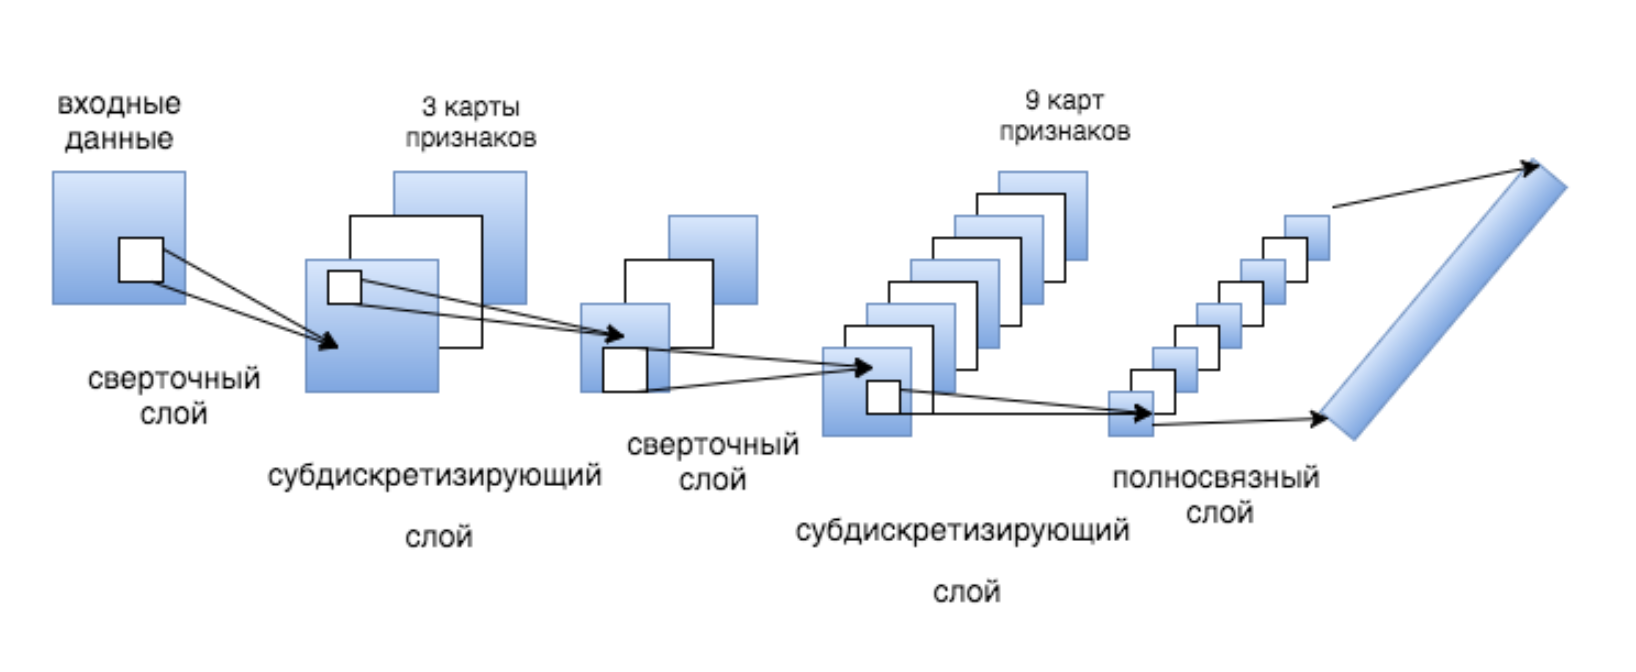
\includegraphics [width=\textwidth*2/3] {images/convnet.png}
    \caption{ Архитектура сверточной нейронной сети}
    \label{fig:convnet}
\end{figure}

\subsubsection{Полносвязный слой} \label{fc_layers}
Слой в котором каждый нейрон соединен со всеми нейронами на предыдущем уровне, причем каждая связь имеет свой весовой коэффициент. На Рис.\ref{fig:fc_layer} показан пример полносвязного слоя.

\begin{figure}[h]
    \centering
    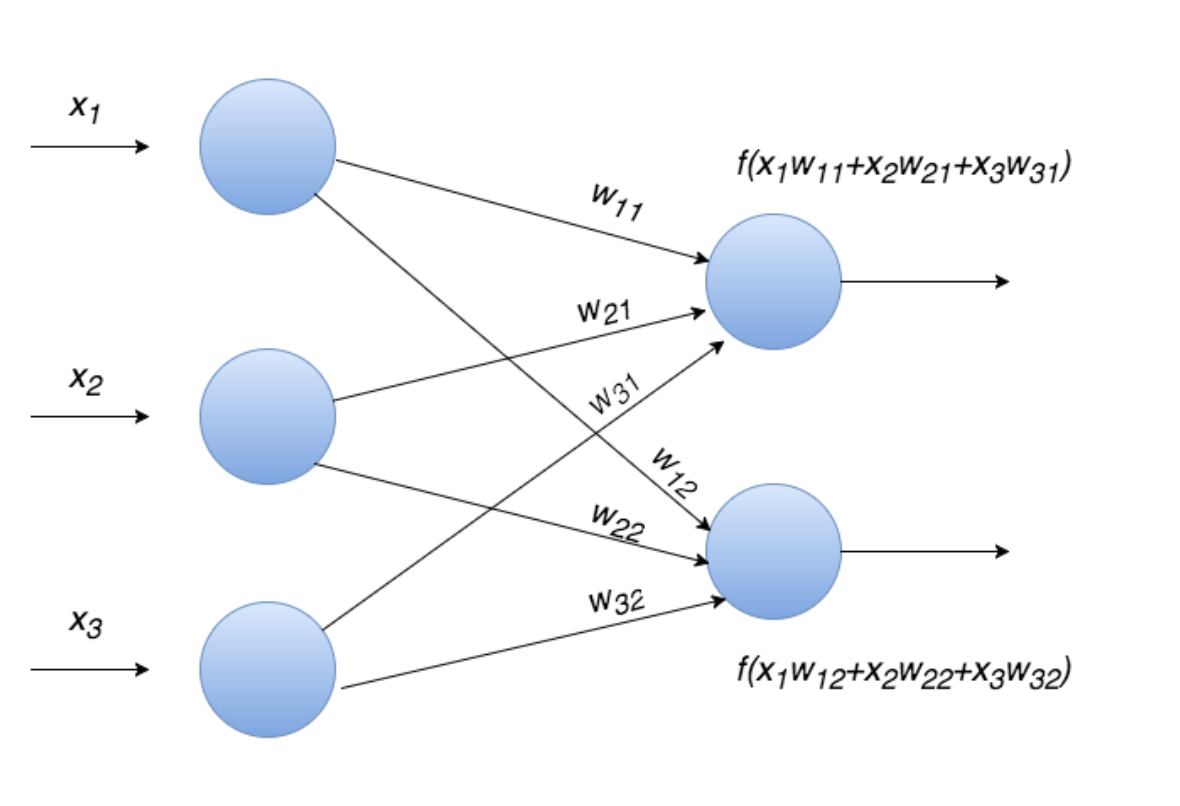
\includegraphics [width=\textwidth*2/3] {images/fc_layer.png}
    \caption{Полносвязный слой}
    \label{fig:fc_layer}
\end{figure}

\begin{itemize}
    \item $w_{i,j}$ — весовые коэффициенты
    \item $f(*)$ — функция активации
\end{itemize}

\subsubsection{Свёрточный слой} \label{conv_layers}
В отличие от полносвязного, в свёрточном слое нейрон соединен лишь с ограниченным количеством нейронов предыдущего уровня, т. е. сверточный слой аналогичен применению операции свертки, где используется лишь матрица весов небольшого размера (ядро свертки), которую «двигают» по всему обрабатываемому слою.

Еще одна особенность свёрточного слоя в том, что он немного уменьшает изображение за счет краевых эффектов.

На Рис. \ref{fig:conv_layer} показан пример сверточного слоя с ядром свертки размера $3 \times 3$.
\begin{figure}[h]
    \centering
    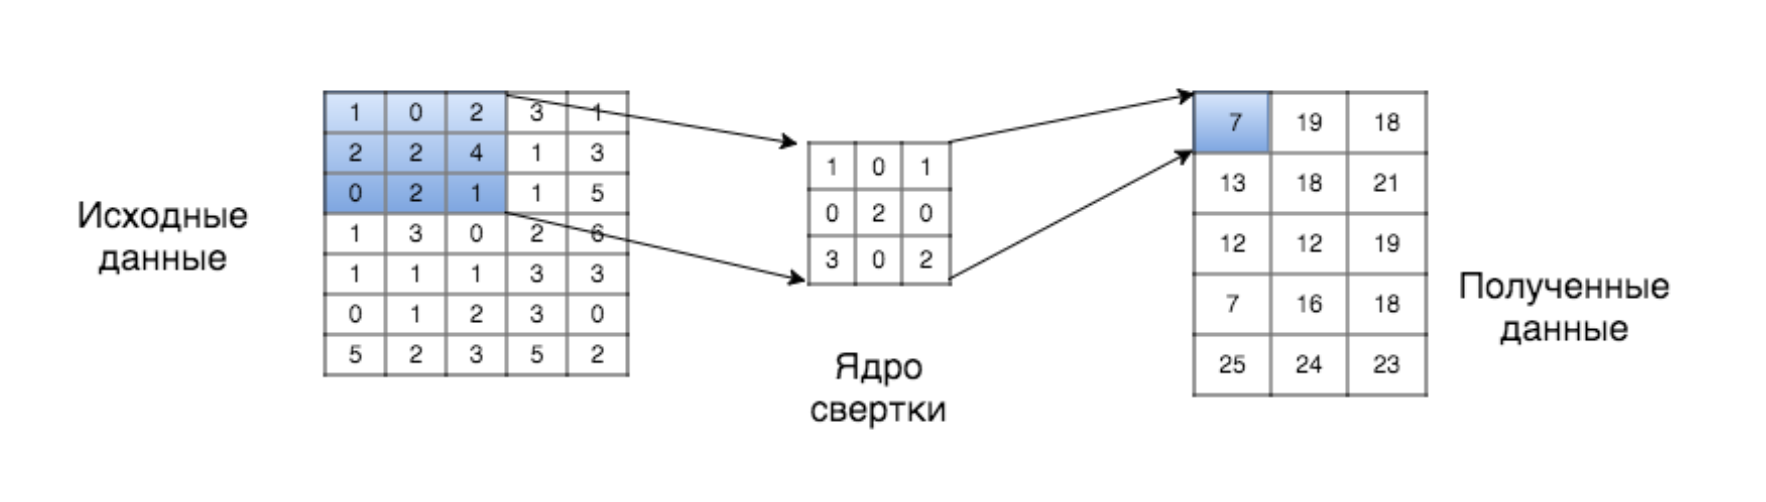
\includegraphics [width=\textwidth*2/3] {images/conv_layer.png}
    \caption{Сверточный слой}
    \label{fig:conv_layer}
\end{figure}

\subsubsection{Cубдискретизирующий слой} \label{pooling_rev}
Слои этого типа выполняют уменьшение размерности (обычно в несколько раз). Это можно делать разными способами, но зачастую используется метод выбора максимального элемента (max-pooling) — вся карта признаков разделяется на ячейки, из которых выбираются максимальные по значению.

На Рис. \ref{fig:pooling_layer} показан пример субдискретизирующего слоя с методом выбора максимального элемента.
\begin{figure}[h]
    \centering
    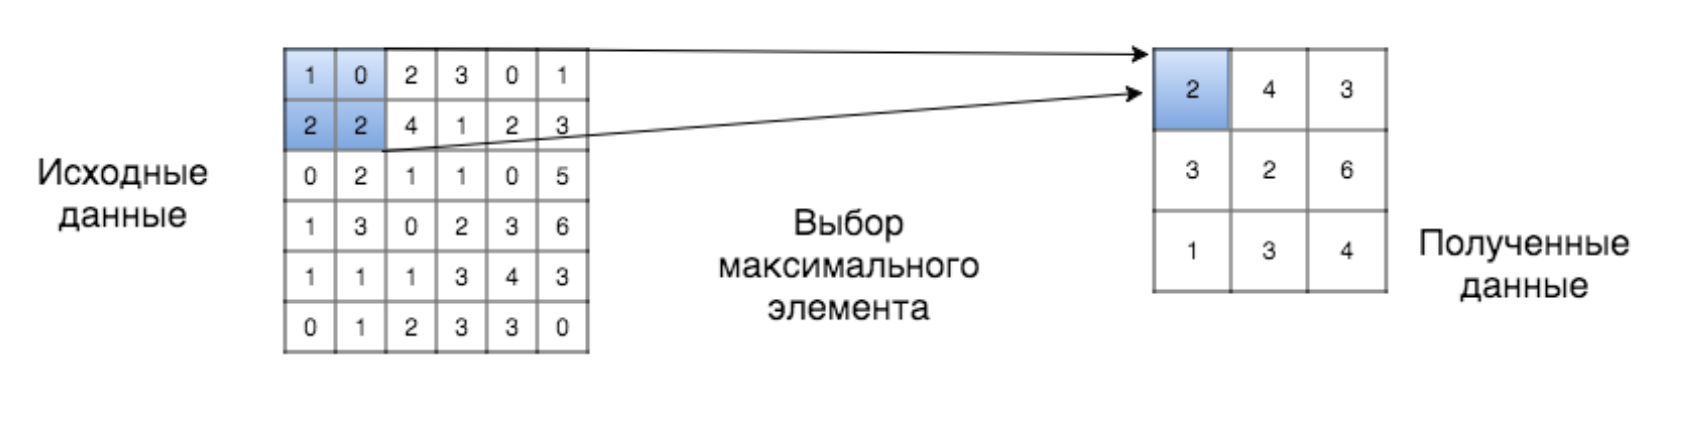
\includegraphics [width=\textwidth*2/3] {images/pooling_layer.png}
    \caption{Cубдискретизирующий слой}
    \label{fig:pooling_layer}
\end{figure}

\subsubsection{Dropout слой} \label{dropout_rev}
Dropout слой (dropout регуляризация)\cite{dropout} способ борьбы с переобучением в нейронных сетях, обучение которых обычно производят стохастическим градиентным спуском, случайно выбирая некоторые объекты из выборки. 

Dropout регуляризация заключается в изменении структуры сети: каждый нейрон выбрасывается с некоторой вероятностью $p$. По такой прореженной сети производится обучение, для оставшихся весов делается градиентный шаг, после чего все выброшенные нейроны возвращаются в нейросеть.

Таким образом, на каждом шаге стохастического градиента мы настраиваем одну из возможных $2N$ архитектур сети, где под архитектурой мы понимаем структуру связей между нейронами, а через $N$ обозначаем суммарное число нейронов. При тестировании нейросети нейроны уже не выбрасываются, но выход каждого нейрона умножается на $(1 - p)$ - благодаря этому на выходе нейрона мы будем получать математическое ожидание его ответа по всем $2N$ архитектурам. Таким образом, нейросеть, обученную с помощью dropout-регуляризации, можно рассматривать как результат усреднения $2N$ сетей.

\subsection{Реализации свёрточных нейронных сетей} \label{nn_archs_lit}
Теперь рассмотрим архитектуры нейронных сетей, которые будут использоваться далее в работе.

\subsubsection{ResNet} \label{resnet_rev}

В 2015 году ResNet произвела настоящую революцию глубины нейросетей. Она состояла из 152 слоёв и снизила процент ошибок до 3,57\%\cite{resnet} в соревновании классификации ImageNet.

Что происходит с нейросетью, при увеличении количества слоёв? Можно ли, взяв обычную архитектуру как AlexNet, просто складывать всё больше и больше слоёв друг на друга и достигать лучшей точности? 

Авторы ResNet в статье описали, что нельзя. Скорее всего, более глубокая нейросеть покажет даже худшие результаты как при обучении, так и при тестировании. И это будет не из-за переобучения, поскольку тогда тренировочная ошибка была бы низкой, см Рис \ref{fig:train_error_deep_net}.

\begin{figure} [h]
    \centering
    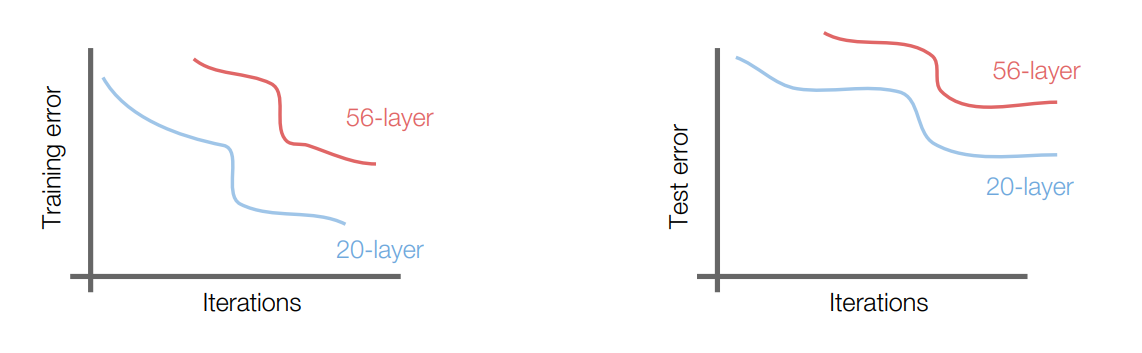
\includegraphics[width=\textwidth*2/3]{images/train_error_deep_net.png}
    \caption{Ошибка на обучающей и тестовой выборке у сети с 20 слоями и 56 слоями}
    \label{fig:train_error_deep_net}
\end{figure}

Создатели ResNet предположили, что узкое место глубоких нейронных сетей кроется в оптимизации — более глубокие модели гораздо хуже поддаются настройке. Тогда они решили не складывать слои друг на друга для изучения отображения нужной функции напрямую, а использовать остаточные блоки, которые пытаются «подогнать» это отображение. Так ResNet стала первой остаточной нейронной сетью\cite{resnet}. Говоря простыми словами, она «перепрыгивает» через некоторые слои. Они больше не содержат признаков и используются для нахождения остаточной функции $H(x) = F(x) + x$ вместо того, чтобы искать $H(x)$ напрямую.

\begin{figure}
    \centering
    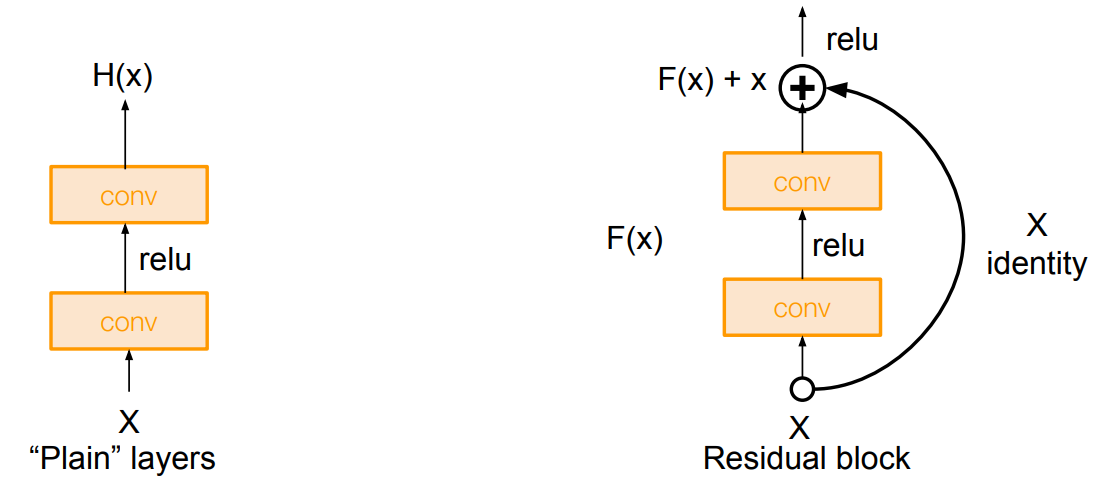
\includegraphics[width=\textwidth*2/3]{images/res_block.png}
    \caption{Обычный слой свёртки и остаточный блок у ResNet}
    \label{fig:my_label}
\end{figure}


Нейросеть состоит из большого стека одинаковых остаточных блоков, каждый из которых имеет два свёрточных слоя $3 \times 3$. Периодически число фильтров удваивается, а их размерность уменьшается с шагом 2 (2 в каждом измерении). В самом начале архитектуры присутствует дополнительный свёрточный слой. Также у ResNet нет полносвязных слоёв в конце — используется только один слой с выходными классами.

Параметры обучения нейронной сети:
\begin{itemize}
    \item После каждого свёрточного слоя используется пакетная нормализация.
    \item SGD + Momentum 0.9.
    \item Скорость обучения — 0.1, делится на 10 при затухании скорости изменения ошибки.
    \item Размер мини-пакета — 256.
    \item Затухание весов — 1e-5.
    \item Dropout не используется.
\end{itemize}

В результате экспериментов с ResNet выяснилось, что очень глубокие сети действительно можно обучить без ухудшения точности. Нейросеть достигла наименьшей ошибки в задачах классификации, которая превзошла даже человеческий результат.

\subsubsection{MobileNet} \label{mobilenet_rev}
В 2017 году Google создала целый класс эффективных моделей под названием MobileNets для мобильных и встраиваемых приложений технического зрения. Сети MobileNet основаны на легковесной архитектуре, использующей разделяемые по глубине свёртки для построения легких глубоких нейронных сетей. 

Нейронная сеть обладает двумя простыми глобальных гиперпараметрами, которые позволяют выбирать между скоростью вычислений и точностью. Эти гиперпараметры позволяют выбрать правильный размер модели для своего приложения, основываясь на ограничениях проблемы. 

Архитектура демонстрирует высокую производительность по сравнению с другими популярными моделями по классификации ImageNet. Спектр применения включает в себя обнаружение объектов, классификацию, распознавание лиц и крупномасштабную геолокализацию.\cite{mobilenet}

Основная особенность этой архитектуры заключается в наличии операторов сгруппированной свёртки. Она позволяет значительно сократить количество вычислений и параметров у модели \cite{xception}. Рассмотрим этот оператор свёртки более подробно.

Сгруппированная свертка - это вариант свертки, при котором каналы карты входных признаков сгруппированы, а свертка выполняется независимо для каждого сгруппированного канала. Её пример можно увидеть на рисунке \ref{fig:gconv}.

\begin{figure}[h]
    \centering
    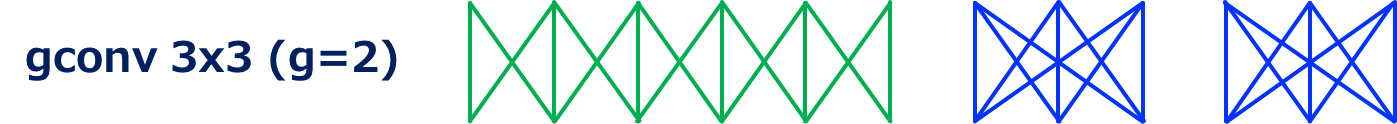
\includegraphics[width=\textwidth*2/3]{images/gconv.png}
    \caption{Сгруппированная свёртка на 5 слоях}
    \label{fig:gconv}
\end{figure}

По сравнению с обычной свёрткой, на рисунке \ref{fig:normal_conv}, можно увидеть что на группированной свёртке слои, разбиваются на две группы, и количество перемножений разительно падает.

\begin{figure}[h]
    \centering
    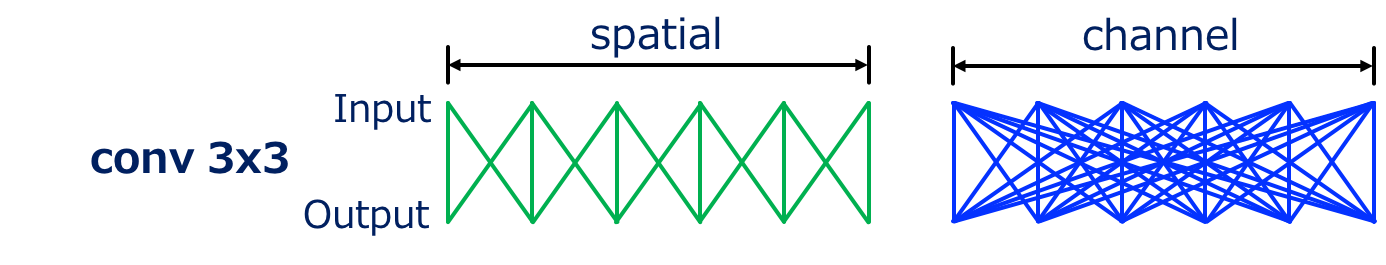
\includegraphics[width=\textwidth*2/3]{images/normal_conv.png}
    \caption{Обычная свёртка на 5 слоях}
    \label{fig:normal_conv}
\end{figure}

Количество вычислений при обычной свёртке:
\[
    Cost = HWNK^2M
\]

где
\begin{itemize}
    \item $Cost$ - Computational Cost или количество вычислений
    \item $H$ - высота изображения
    \item $W$ - высота изображения
    \item $N$ - количество каналов на входе
    \item $K$ - размер ядра свёртки. В квадрате, т.к. высота и ширина ядра обычно равны
    \item $M$ - количество каналов на выходе
\end{itemize}

При сгруппированной свёртке количество вычислений падает пропорционально количеству групп. 
\[
    Cost = \dfrac{HWNK^2M}{G}
\]

где $G$ - это количество групп свёртки.

Когда количество групп свёртки совпадает с количеством слоёв в исходном изображении, такую свёртку называют depthwise convolution или послойная свёртка. Рис \ref{fig:depthwise_conv}.

\begin{figure}[h]
    \centering
    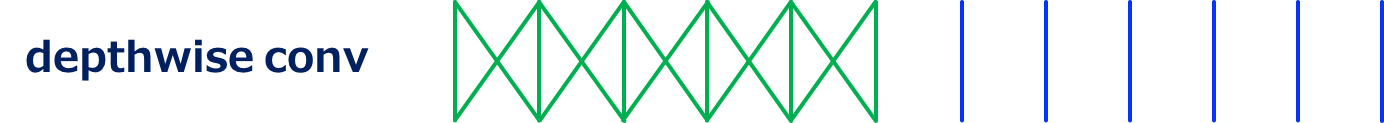
\includegraphics[width=\textwidth*2/3]{images/depthwise_conv.png}
    \caption{Послойная свёртка}
    \label{fig:depthwise_conv}
\end{figure}
